The given system of inequality can be written in matrix form as
\begin{align}
    \myvec{-5 & -4 \\ 1 & 0 \\ 0 & 1}\vec{x} \succeq \myvec{-40\\2\\3}
\end{align}
Let the surplus vector be
\begin{align}
    \vec{u} &= \myvec{u_1\\u_2} \succeq 0
\end{align}
The first pair of inequality can be solved as,
\begin{enumerate}
    \item 
    \begin{align}
        \myvec{-5 & -4 \\ 1 & 0}\vec{x} &\succeq \myvec{-40 \\ 2}
        \\
        \implies  \myvec{-5 & -4 \\ 1 & 0}\vec{x} &= \myvec{-40 \\ 2} + \vec{u}
    \end{align}
    resulting in 
    \begin{align}
        \vec{x} &= \myvec{-5 & -4 \\1 & 0}^{-1}\myvec{-40 \\ 2} + \myvec{-5 & -4 \\1 & 0}^{-1}\vec{u}
        \\
        \implies \vec{x} &= \myvec{2 \\\frac{15}{2}} + \myvec{0 & 1\\ \frac{-1}{4} & \frac{-5}{4}}\vec{u}   \label{aug/2/2eq1}
    \end{align}
    Similarly, solving 2nd pair of inequality
    \item 
    
    \begin{align}
        \myvec{-5 & -4\\ 0 & 1}\vec{x} &\succeq \myvec{-40 \\ 3}
        \\
        \implies  \myvec{-5 & -4 \\ 1 & 0}\vec{x} &= \myvec{-40 \\ 3} + \vec{u}
    \end{align}
    resulting in 
    
    \begin{align}
        \vec{x} &= \myvec{-5 & -4 \\0 & 1}^{-1}\myvec{-40 \\ 3} + \myvec{-5 & -4 \\0 & 1}^{-1}\vec{u}
        \\
        \implies \vec{x} &= \myvec{\frac{28}{5} \\3} + \myvec{\frac{-1}{5} & \frac{-4}{5}\\ 0 & 1}\vec{u} \label{aug/2/2eq2}
    \end{align}
    
\end{enumerate}
Now,solution region which is common to regions of eq. \eqref{aug/2/2eq1} and eq. \eqref{aug/2/2eq2},is given by
\begin{align}
    \boxed{\vec{x} = \myvec{2 \\ 3}+\myvec{0 & 1\\ \frac{1}{20} & \frac{-21}{20}}\vec{u}}
\end{align}
See Fig. \ref{aug/2/2fig:fig1}.
%
\begin{figure}[!ht]
\centering
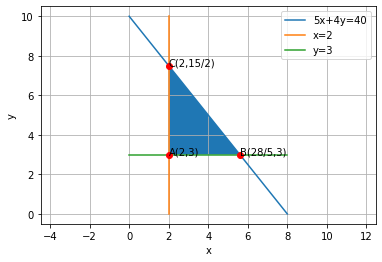
\includegraphics[width=\columnwidth]{solutions/aug/2/2/Figures/Figure1.png}
\caption{Solution Region}
\label{aug/2/2fig:fig1}	
\end{figure}

% \numberwithin{figure}{section}
% \begin{figure}[!ht]
% \centering
% 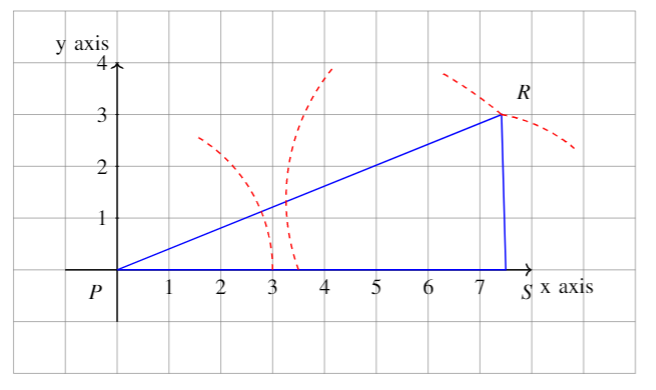
\includegraphics[width=\columnwidth]{Figure2.png}
% \caption{Magnified Solution Region}
% \label{aug/2/2fig:fig2}	
% \end{figure}
